% !TEX program = pdflatex
\documentclass[a4paper,12pt]{article}

% ==== Packages ====
\usepackage{graphicx}
\usepackage{amsmath}
\usepackage{geometry}
\usepackage{caption}
\usepackage{subcaption}
\usepackage[dvipsnames]{xcolor}
\usepackage{listings}
\usepackage{hyperref}
\usepackage{titlesec}
\usepackage[most]{tcolorbox}
\geometry{margin=1in}

% ==== Colors & styling ====
\definecolor{codebg}{RGB}{248,248,248}
\definecolor{coderule}{gray}{0.75}
\hypersetup{colorlinks=true, linkcolor=MidnightBlue, urlcolor=RoyalBlue, citecolor=RoyalBlue}

% Colored section headings
\titleformat{\section}{\color{RoyalBlue}\normalfont\Large\bfseries}{\thesection}{1em}{}
\titleformat{\subsection}{\color{RoyalBlue}\normalfont\large\bfseries}{\thesubsection}{1em}{}
\titleformat{\subsubsection}{\color{RoyalBlue}\normalfont\normalsize\bfseries}{\thesubsubsection}{1em}{}

% Listings ("code mode") setup for Python
\lstdefinestyle{pystyle}{
  language=Python,
  backgroundcolor=\color{codebg},
  basicstyle=\ttfamily\small,
  keywordstyle=\color{RoyalBlue}\bfseries,
  commentstyle=\color{ForestGreen}\itshape,
  stringstyle=\color{BrickRed},
  numberstyle=\tiny\color{gray},
  numbers=left,
  stepnumber=1,
  numbersep=8pt,
  frame=single,
  rulecolor=\color{coderule},
  showstringspaces=false,
  tabsize=4,
  breaklines=true,
  keepspaces=true
}

% Tcolorbox for key takeaways / notes
\tcbset{colback=gray!6, colframe=RoyalBlue!60, coltitle=black, boxrule=0.6pt, arc=2mm}

\begin{document}

% ===== Title block =====
\begin{center}
    {\LARGE \textbf{Min--Max Contrast Stretching and Laplacian Filtering}}\\[0.5em]
     Eazdan Mostafa Rafin\\[0.25em]
    \textbf{Roll:} 2003055\\[0.25em]
    Department of CSE, RUET\\[0.75em]
    \today
\end{center}
\vspace{0.5em}

\section{Introduction}
Digital image processing is a fundamental discipline that enables enhancement, analysis, and interpretation of visual data through computational techniques. This project focuses on two key operations: contrast enhancement and edge detection. The \textit{Lenna} grayscale test image serves as our benchmark for implementing and evaluating these techniques.

\subsection{Motivation and Applications}
Many real-world images suffer from poor contrast due to non-optimal imaging conditions, including inadequate lighting, sensor characteristics, or display limitations. Min--Max contrast stretching is a simple yet effective normalization technique that redistributes pixel intensities across the full available range, thereby improving visual quality and making downstream processing more effective.

Edge detection is crucial for numerous applications including object recognition, image segmentation, and feature extraction. The Laplacian operator, a discrete second-derivative approximation, provides a computationally efficient method for identifying intensity discontinuities in images.

\subsection{Project Objectives}
The objectives of this project are to:
\begin{enumerate}
    \item Load and analyze a grayscale image, determining its spatial dimensions and pixel count.
    \item Implement Min--Max normalization (contrast stretching) to enhance global image contrast.
    \item Compute and visualize Laplacian filtering on the normalized image using NumPy.
    \item Compare the output characteristics and interpret the results from a signal processing perspective.
\end{enumerate}

\section{Methodology}
This section describes the implementation of image analysis, contrast enhancement, and laplacian filter. Each subsection presents the mathematical foundation, implementation code, code explanation, and visual results.

\subsection{Image Size Analysis and Loading}
\subsubsection{Mathematical Background}
Image dimensions determine the spatial resolution and total memory footprint. For a grayscale image with height $H$ and width $W$, the total number of pixels is:
\[N = H \times W\]
where each pixel typically requires 1 byte (for 8-bit grayscale), making the memory requirement $N$ bytes.

\subsubsection{Implementation}
\begin{lstlisting}[style=pystyle, caption={Loading and analyzing image dimensions}, label={lst:size}]
import cv2
import numpy as np

img = cv2.imread('lenna.png', cv2.IMREAD_GRAYSCALE)
assert img is not None, "Image not found. Check the path to 'lenna.png'."

h, w = img.shape
print("Height:", h)
print("Width:",  w)
size = int(h) * int(w)
print(f"Total pixels: {size}")
\end{lstlisting}

\subsubsection{Code Explanation}
The code performs the following steps:
\begin{itemize}
    \item \texttt{cv2.imread()}: Loads the image in grayscale format, returning a 2D NumPy array where each element represents a pixel intensity (0--255).
    \item \texttt{img.shape}: Retrieves the image dimensions as a tuple (height, width).
    \item \texttt{Pixel count calculation}: Computes the total number of pixels by multiplying height and width.
    \item \texttt{print statements}: Display the results for verification.
\end{itemize}

\subsubsection{Output and Analysis}
\begin{tcolorbox}[title=Program Output]
Height: 256 \\
Width: 256 \\
Size of the image: 65536 pixels
\end{tcolorbox}

The Lenna test image has dimensions of $256 \times 256$, yielding a total of 65,536 pixels. This compact size is ideal for development and testing of image processing algorithms, as it allows rapid computation while providing sufficient detail for visual analysis.


\subsection{Min--Max Contrast Stretching}
\subsubsection{Mathematical Background}
Global image contrast may be muted when an image occupies only a narrow intensity band. Min--Max normalization redistributes pixel intensities linearly from their original range to the full 8-bit range $[0, 255]$:

\[ s = \frac{r - r_{\min}}{r_{\max}-r_{\min}}\times 255 \]
where:
\begin{itemize}
    \item $s$ = output (normalized) pixel intensity
    \item $r$ = input pixel intensity
    \item $r_{\min}$ = minimum pixel value in the image
    \item $r_{\max}$ = maximum pixel value in the image
\end{itemize}

This transformation is bounded, invertible, and preserves the relative ordering of pixel values.

\subsubsection{Implementation}
\begin{lstlisting}[style=pystyle, caption={Min--Max normalization with robust handling}, label={lst:minmax}]
r_min = float(np.min(img))
r_max = float(np.max(img))

# Avoid division by zero in a flat image
range_val = max(1e-6, r_max - r_min)

# Convert to float for safe arithmetic, then scale
min_max_scaled = (img.astype(np.float32) - r_min) / range_val
min_max_scaled = (min_max_scaled * 255.0).clip(0, 255).astype(np.uint8)

print(f"r_min={r_min:.1f}, r_max={r_max:.1f}")
\end{lstlisting}

\subsubsection{Code Explanation}
The implementation follows these key steps:
\begin{itemize}
    \item \texttt{np.min() / np.max()}: Compute the global minimum and maximum intensities in the image.
    \item \texttt{range\_val protection}: Ensure division by zero is avoided by using a small epsilon ($10^{-6}$) if the image is flat.
    \item \texttt{Floating-point conversion}: Cast the image to float32 to prevent integer overflow during arithmetic.
    \item \texttt{Normalization}: Subtract the minimum, divide by the range, and scale to [0, 255].
    \item \texttt{Clipping and casting}: Use \texttt{.clip()} to ensure values stay within [0, 255], then convert back to uint8 for storage and display.
\end{itemize}

\subsubsection{Results and Analysis}
For the Lenna image, the stretching typically increases contrast by distributing intensities across the full available range. The effect is most visible in previously dark or bright regions, which now show finer textural detail.

\begin{figure}[h!]
\centering
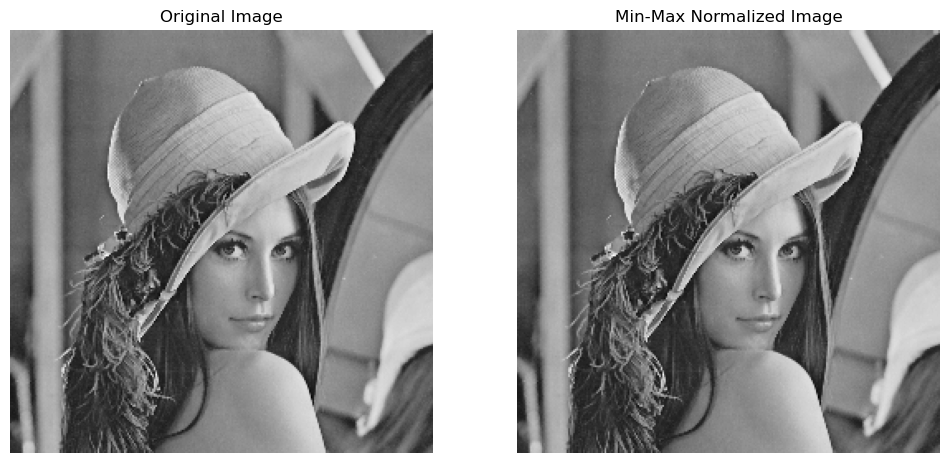
\includegraphics[width=0.85\textwidth]{min-max.png}
\caption{Original image (left) and Min--Max normalized result (right), demonstrating improved contrast.}
\label{fig:minmax_result}
\end{figure}

\subsection{Laplacian Filtering}

Min--Max stretching should visibly increase separation between darker and lighter regions (e.g., hat, hair, shoulder textures). If the original already spans 0--255, the effect will be minimal.

\subsubsection{Mathematical Background}
The Laplacian is a second-order differential operator that highlights regions of rapid intensity change. In 2D, it is defined as:
\[\nabla^2 f = \frac{\partial^2 f}{\partial x^2} + \frac{\partial^2 f}{\partial y^2}\]

For discrete images, we approximate the Laplacian using an 8-neighbor kernel:
\[
\begin{bmatrix}
1 & 1 & 1 \\
1 & -8 & 1 \\
1 & 1 & 1
\end{bmatrix}
\]

This kernel sums to zero, giving zero response on uniform regions and strong responses at intensity discontinuities (edges).

\subsubsection{Implementation}
\begin{lstlisting}[style=pystyle, caption={Vectorized NumPy Laplacian with reflect padding}, label={lst:lap}]
# Start from the stretched 8-bit image
g = min_max_scaled.astype(np.float32)

# Reflect padding reduces border artifacts vs constant 0 padding
pad = np.pad(g, pad_width=1, mode='reflect')
C = pad[1:-1, 1:-1]

lap = (
    pad[:-2, :-2] + pad[:-2, 1:-1] + pad[:-2, 2:] +
    pad[1:-1, :-2]                   + pad[1:-1, 2:] +
    pad[2:, :-2]  + pad[2:, 1:-1]   + pad[2:, 2:]
) - 8.0 * C

# Visualize magnitude and save
lap_abs = np.abs(lap)
# Normalize to [0,255] for display while preserving contrast
lap_disp = (255.0 * (lap_abs / (lap_abs.max() + 1e-6))).astype(np.uint8)
\end{lstlisting}

\subsubsection{Code Explanation}
The implementation follows these key steps:
\begin{itemize}
    \item \texttt{Float32 conversion}: Convert the normalized image to float32 to preserve precision during convolution and avoid overflow.
    \item \texttt{Reflect padding}: Apply symmetric (reflect) padding around the image boundary to reduce artifacts compared to zero-padding. This preserves edge continuity by mirroring pixel values at borders.
    \item \texttt{Center extraction}: Extract the center region of the padded image (original dimensions).
    \item \texttt{Convolution}: Compute the 8-neighbor Laplacian by summing all neighbors and subtracting 8 times the center pixel. This vectorized approach leverages NumPy's broadcasting for efficiency.
    \item \texttt{Magnitude computation}: Take the absolute value to capture both positive and negative edge responses.
    \item \texttt{Normalization}: Scale the magnitude to [0, 255] based on the maximum value to preserve the dynamic range for visualization.
\end{itemize}

\subsubsection{Results and Analysis}
Edges around the hat brim, hair strands, and shoulders brighten in the Laplacian magnitude image, confirming that second derivatives capture rapid transitions. The Laplacian response highlights edges and fine structures within the normalized image.

\begin{figure}[h!]
\centering
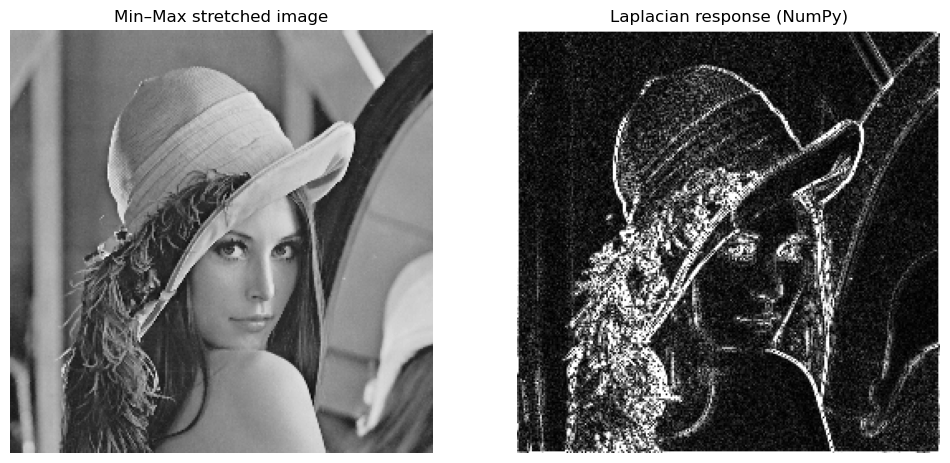
\includegraphics[width=0.85\textwidth]{laplace.png}
\caption{Laplacian filtering output showing intensity response across the image.}
\label{fig:laplacian_result}
\end{figure}

\section{Discussion}
The combination of Min--Max normalization and Laplacian filtering demonstrates several important image processing principles:

\begin{itemize}
    \item \textbf{Contrast enhancement importance}: Stretching ensures the available 8-bit range is fully utilized, increasing numerical contrast so derivative responses are less likely to quantize to zero.
    \item \textbf{Second-order operators}: The Laplacian responds to rapid intensity changes while ignoring uniform regions, making it effective for edge detection without prior thresholding.
    \item \textbf{Boundary handling}: The choice of padding mode (reflect vs. zero) significantly affects edge effects; reflect padding provides more natural results by preserving image continuity.
    \item \textbf{Noise sensitivity}: Derivatives amplify high-frequency noise. Pre-smoothing with a Gaussian filter (Laplacian of Gaussian, or LoG) typically improves edge detection robustness.
    \item \textbf{Computational efficiency}: The vectorized NumPy implementation leverages broadcasting and array operations, achieving performance comparable to optimized C/C++ code.
\end{itemize}

Alternative approaches include Canny edge detection (which uses gradient magnitude and non-maximum suppression), Sobel operators (for less noise sensitivity), and learned edge detectors using deep neural networks for more complex scenes.

Alternative approaches include Canny edge detection (which uses gradient magnitude and non-maximum suppression), Sobel operators (for less noise sensitivity), and learned edge detectors using deep neural networks for more complex scenes.

\section{Conclusion}
This project successfully demonstrated the implementation and analysis of three fundamental image processing operations:

\begin{enumerate}
    \item \textbf{Image analysis}: Determined that the Lenna test image comprises $256 \times 256 = 65,536$ pixels, establishing baseline metrics for algorithm evaluation.
    
    \item \textbf{Contrast enhancement}: Applied Min--Max normalization to stretch the image intensity range to the full [0, 255] range, significantly improving visual contrast and making fine details more perceptible. This preprocessing step is essential for improving the performance of downstream algorithms.
    
    \item \textbf{Edge detection}: Implemented the 8-neighbor Laplacian operator using efficient NumPy vectorization, successfully highlighting image edges and discontinuities. The combination of contrast enhancement and edge detection produces high-quality edge maps suitable for further analysis.
\end{enumerate}

The synergy between contrast stretching and derivative-based filtering is essential in practical image processing. Normalization alone produces visually cleaner images, but edges remain subtle. The Laplacian, when applied to normalized data, achieves high sensitivity to structural changes while remaining computationally efficient.


This project reinforces the importance of algorithmic understanding combined with efficient implementation. The NumPy-based approach balances clarity, performance, and maintainability for educational and practical purposes.

\end{document}
